    The real world is composed of geometrical objects and our models for physics, chemistry, and biology rely heavily on utilizing them.  But, how can one describe certain objects such as a sphere, a donut, or a helical curve?  We have seen these types of surfaces arise in a few ways, but we need something that provides us a more pragmatic approach to constructing such objects. The two means we will look at in this chapter are that of \boldgreen{implicit} and \boldgreen{explicit parameterizations}. First and foremost, a \boldgreen{parameterization} is a means in which one can describe a geometrical object via variables.  For example, one could describe the unit sphere as the level set to $x^2+y^2+z^2=1$ or one could describe a parabaloid via the graph of the function $z=x^2+y^2$. The former is an example of an implicit paramaterization while the latter is explicit. Let's briefly discuss the differences between these approaches.

    Let us now consider surfaces in $\R^3$ as the prototypical example for a need for providing a parameterization.  To be a bit more precise, a surface is a 2-dimensional membrane that lives inside of space.  It is not a bad idea to picture a sphere, a donut, or a wiggly sheet of rubber. In general, an implicit parameterization of a surface is given by a list of equations of functions of more than two variables.  For example, if we consider
    \[
    f(x,y,z) = x^2+y^2+z^2,
    \]
    then we take
    \[
    f(x,y,z) = 1,
    \]
    this gives us a spherical surface.  Notice how $f(x,y,z)$ depends on three variables, and setting this equation equal to a constant gives us a surface.  There is a far more general approach where we may consider a list of functions $f_1(x_1,x_2,\dots,x_n)$, $f_2(x_1,x_2,\dots,x_n)$, $\dots$, $f_m(x_1,x_2,\dots,x_n)$ where we set each of these functions equal to a constant. For example,
    \begin{align*}
        f_1(x_1,x_2,\dots,x_n) &= c_1\\
        f_2(x_1,x_2,\dots,x_n) &= c_2\\
        &\vdots\\
        f_m(x_1,x_2,\dots,x_n) &= c_m.
    \end{align*}
    However, we will not need such abstraction.

    In the explicit case, we provide a different perspective.  Namely, we seek to describe the two dimensional membrane using two variables $u$ and $v$, and we take the functions $x(u,v)$, $y(u,v)$, and $z(u,v)$ to describe the points in space that live on this surface.  That is, if $u\in [u_0,u_1]$ and $v\in [v_0,v_1]$, then a surface can be described by the set of points
    \[
    (x(u,v),y(u,v),z(u,v)).
    \]
    This description is a bit more abstract than we wish.  For us, we will take surfaces to be broken up into graphs.  For example, we could take the surface given by the points
    \[
    (x,y,f(x,y)),
    \]
    where $f(x,y)=x^2+y^2$ to receive the parabaloid surface.  Notice that here we have swapped $u$ and $v$ for $x$ and $y$ since we are able to construct this as a graph. Graphs are simply the nicest examples of explicit surfaces.


\section{Implicit  surfaces}
                In the planar case, we would often have to specify a set of points by providing an equation
                \[
                x^2+y^2=1.
                \]
                The tuples of points $(x,y)$ which satisfy the above equations define a nice set of points in the plane that we know as the unit circle.

                \begin{exercise}
                	Verify that the set of points $(x,y)$ is indeed the unit circle. \emph{Hint: you can take the points to be $(\cos(\theta),\sin(\theta))$ for $\theta \in [0,2\pi)$ and notice that these points all live on the circle. Is it possible to find other points?}
                 \end{exercise}

                This concept should not be totally foreign to us as we previously worked with level sets of scalar fields.  The above example is nothing but the 1 level set to the function $f(x,y)=x^2+y^2$.  In higher dimensions, we can do the same in order to visualize functions of the form $f\colon \R^3\to \R$ written as $f(x,y,z)$.  If we pick some constant $c$ and write
                \[
                f(x,y,z)=c
                \]
                then we will get level surfaces for the function $f(x,y,z)$.  We should also remark that surfaces are common objects in space, and we would like a means of describing them anyways. We refer to this description of level surfaces as \boldgreen{implicit}. Some even refer to these surfaces as \boldgreen{implicit surfaces}.  Later, we will also consider explicit parameterizations.

                \begin{ex}{A Sphere as a Level Surface}{sphere_lev_surf}
                We can consider the following function
                \[
                f(x,y,z)=x^2+y^2+z^2.
                \]
                If we take the one level set, that is the points $(x,y,z)$ that satisfy
                \[
                x^2+y^2+z^2=1
                \]
                then we get the unit \boldgreen{sphere}.  These are the set of points that are all a distance one from the origin.
              	\begin{figure}[H]
              		\centering
              		\includegraphics[width=.8\textwidth]{Figures_Part_6/Sphere.png}
              		\caption{The unit sphere in $\R^3$ as the solution to $x^2+y^2+z^2=1$.}
              	\end{figure}

              	If we change the constant from $c=1$, the surface will also change.  That is, if we consider the equation
              	\[
              	f(x,y,z)=c,
              	\]
              	then each $c$ describes a different set of points.  Let's investigate and see what our options are.

              	It's quite clear that $c\geq 0$ since a $c$ value less than zero will have no real solutions.  One should make sure this is clear.  For the value $c=0$, we have
              	\[
              	x^2+y^2+z^2=0,
              	\]
              	which has a single solution of $(x,y,z)=(0,0,0)$.  Thus, the level set for $c=0$ is not a surface but a single point.  For values $c>0$, we will define a sphere with radius $\sqrt{c}$.  Note that the distance from the origin to any point in the plane $(x,y,z)$ is defined by
              	\[
              	\sqrt{x^2+y^2+z^2},
              	\]
              	and so this description of the sphere is capturing the distance from the origin to a point on the sphere.  Calling this distance
              	\[
              	r=\sqrt{x^2+y^2+z^2},
              	\]
              	we have that
              	\[
              	r^2 = c ~ \implies~ r = \sqrt{c}.
              	\]
                \end{ex}

                The sphere will be a go-to example of an implicit surface.  The function that describes the sphere behaves rather nicely and the sphere also provides a great visualization.  Later on, we will cover a new system of coordinates in $\R^3$ that is based upon the sphere as well.

                One may wonder what happens at the origin in the previous example.  To see the issue, we can consider the gradient of the scalar field that defined the surface, $f(x,y,z) = x^2+y^2+z^2$.  Taking the gradient yields,
                \[
                \grad f = \begin{pmatrix} 2x \\ 2y \\ 2z \end{pmatrix}.
                \]
                If we evaluate the gradient at the origin, we can note
                \[
                \grad f(0,0,0) = \begin{pmatrix} 0 \\ 0 \\ 0 \end{pmatrix},
                \]
                which is the zero vector!  This leads us to the following.

                \begin{thm}{Implicit Surfaces iff $\grad f \neq 0$}{implicit_surfaces_gradient}
                	Given a scalar field $f(x,y,z)$, the equation $f(x,y,z)=c$ defines an implicit surface if the gradient $\grad f$ on the level set of points ($\{(x,y,z) \in \R^3 ~\vert~ f(x,y,z)=c\}$) does not vanish. Thus, if we take a level set and consider the points where the gradient is nonzero, we have a level surface.
                \end{thm}

                \begin{ex}{The Hyperboloids}{hyperboloids}
                If we change the function above just slightly, we will receive a whole family of surfaces given by the level sets of
                \[
                f(x,y,z)=x^2+y^2-z^2.
                \]
                Again, we will have to consider what values for $c$ define level surfaces.
                \begin{itemize}
                    \item If we take $c=0$ and set
                    \[
                    x^2+y^2-z^2=0.
                    \]
                    then we find the 0 level surface. In this case, we can do a bit of work to find
                    \[
                    z=\pm \sqrt{x^2+y^2}.
                    \]
                    Notice, if we pick any value for $z$, that we get a circle at that level!  When $z=0$, we get a single point.  It turns out that we get the \boldgreen{(double) cone} surface which looks like
                    \begin{figure}[H]hy
                        \centering
                     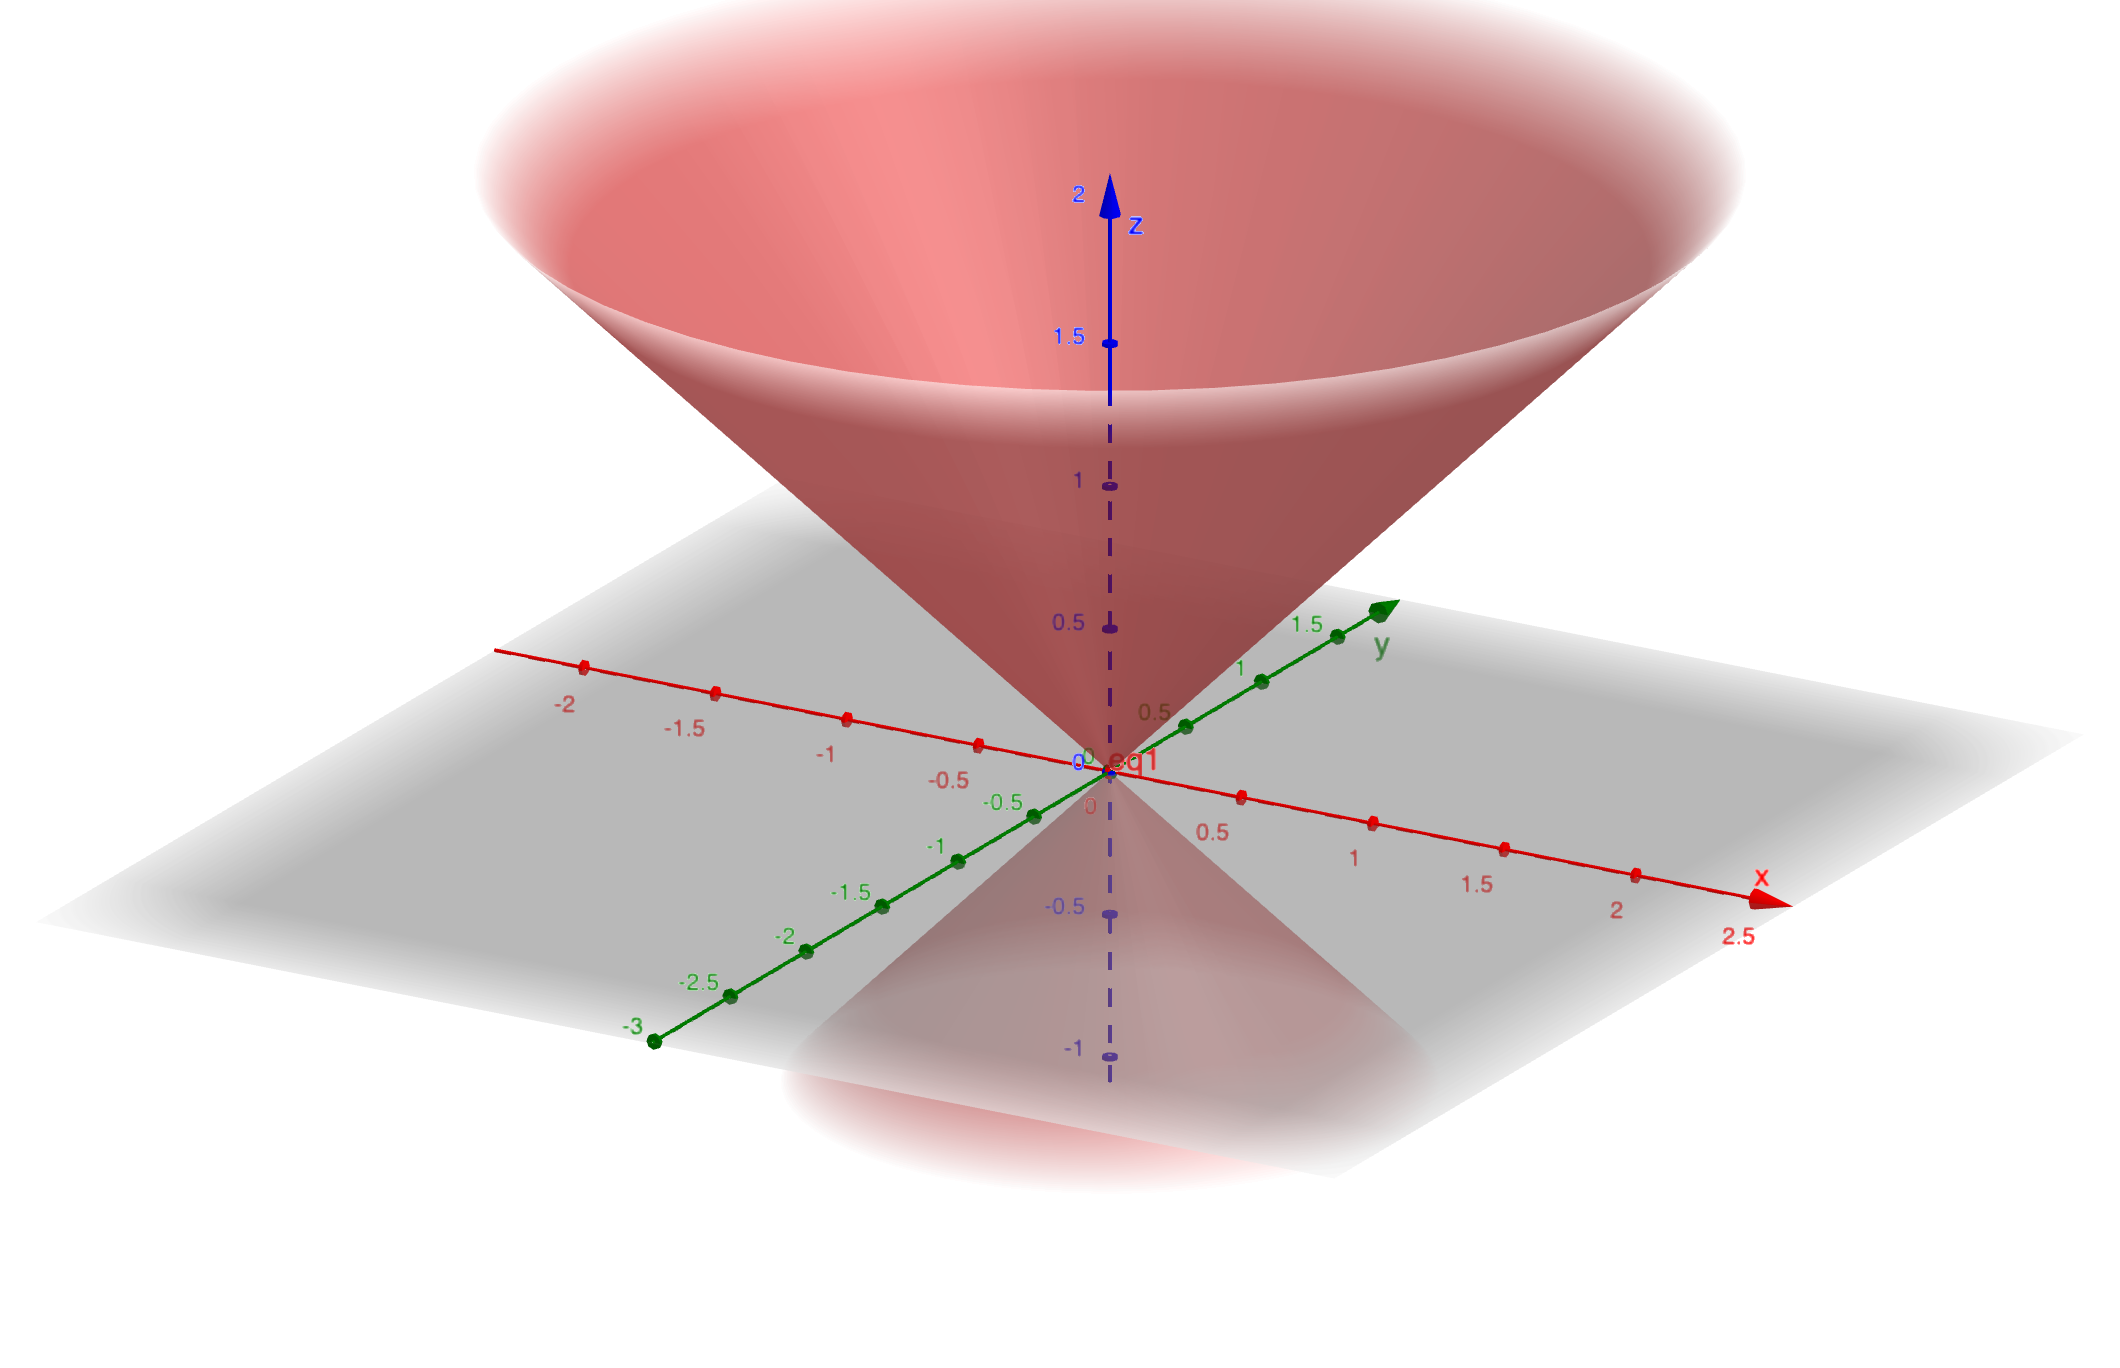
\includegraphics[width=.8\textwidth]{Figures_Part_6/cone_surface.png}
                     \caption{(Double) cone surface given by the level set $c=0$.}
                    \end{figure}
                    At the origin, $(x,y,z)=(0,0,0)$, we can see that our surface degenerates to a single point. Again, one can see that the gradient at that point $\grad f(0,0,0) = \zerovec$.

                    One should take some time to work out visualizing this both with software like GeoGebra as well as by hand.

                    \item If we take $c=1$ and set
                    \[
                    x^2+y^2-z^2=1
                    \]
                    we get the \emph{hyperboloid of one sheet}.  This looks like
                    \begin{figure}[H]
                        \centering
                        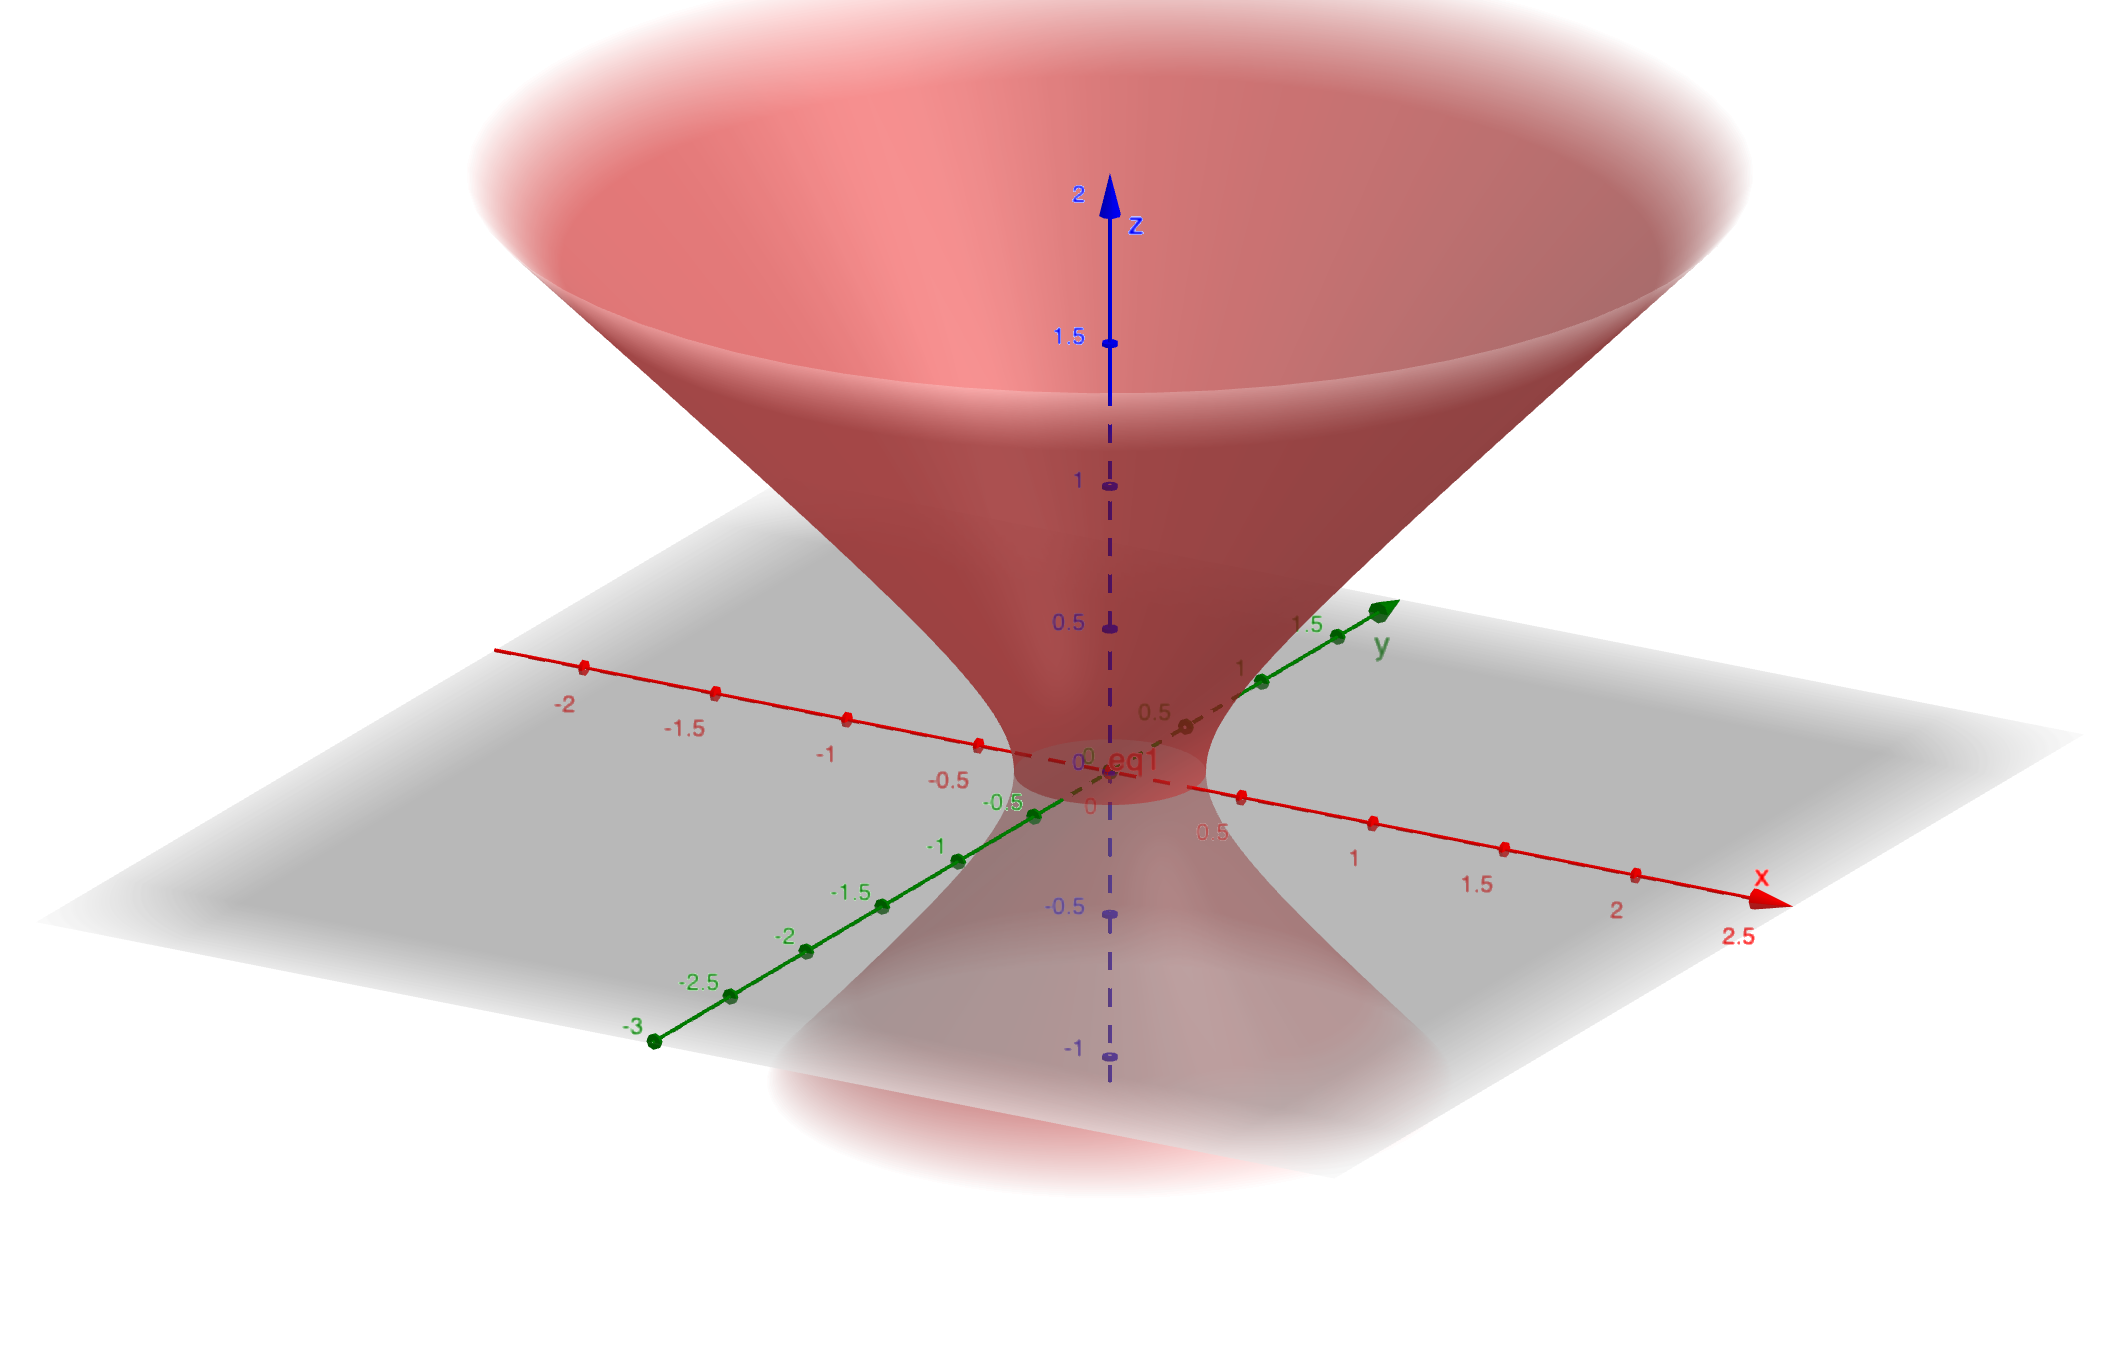
\includegraphics[width=.8\textwidth]{Figures_Part_6/hyperboloid_1_sheet.png}
                        \caption{Hyperboloid of 1-sheet defined by $c=0.1$.}
                    \end{figure}

                    \item If we take $c<0$ and set
                    \[
                    x^2+y^2-z^2=c
                    \]
                    we get a \boldgreen{hyperboloid of two sheets}.  This looks like
                    \begin{figure}[H]
                        \centering
                        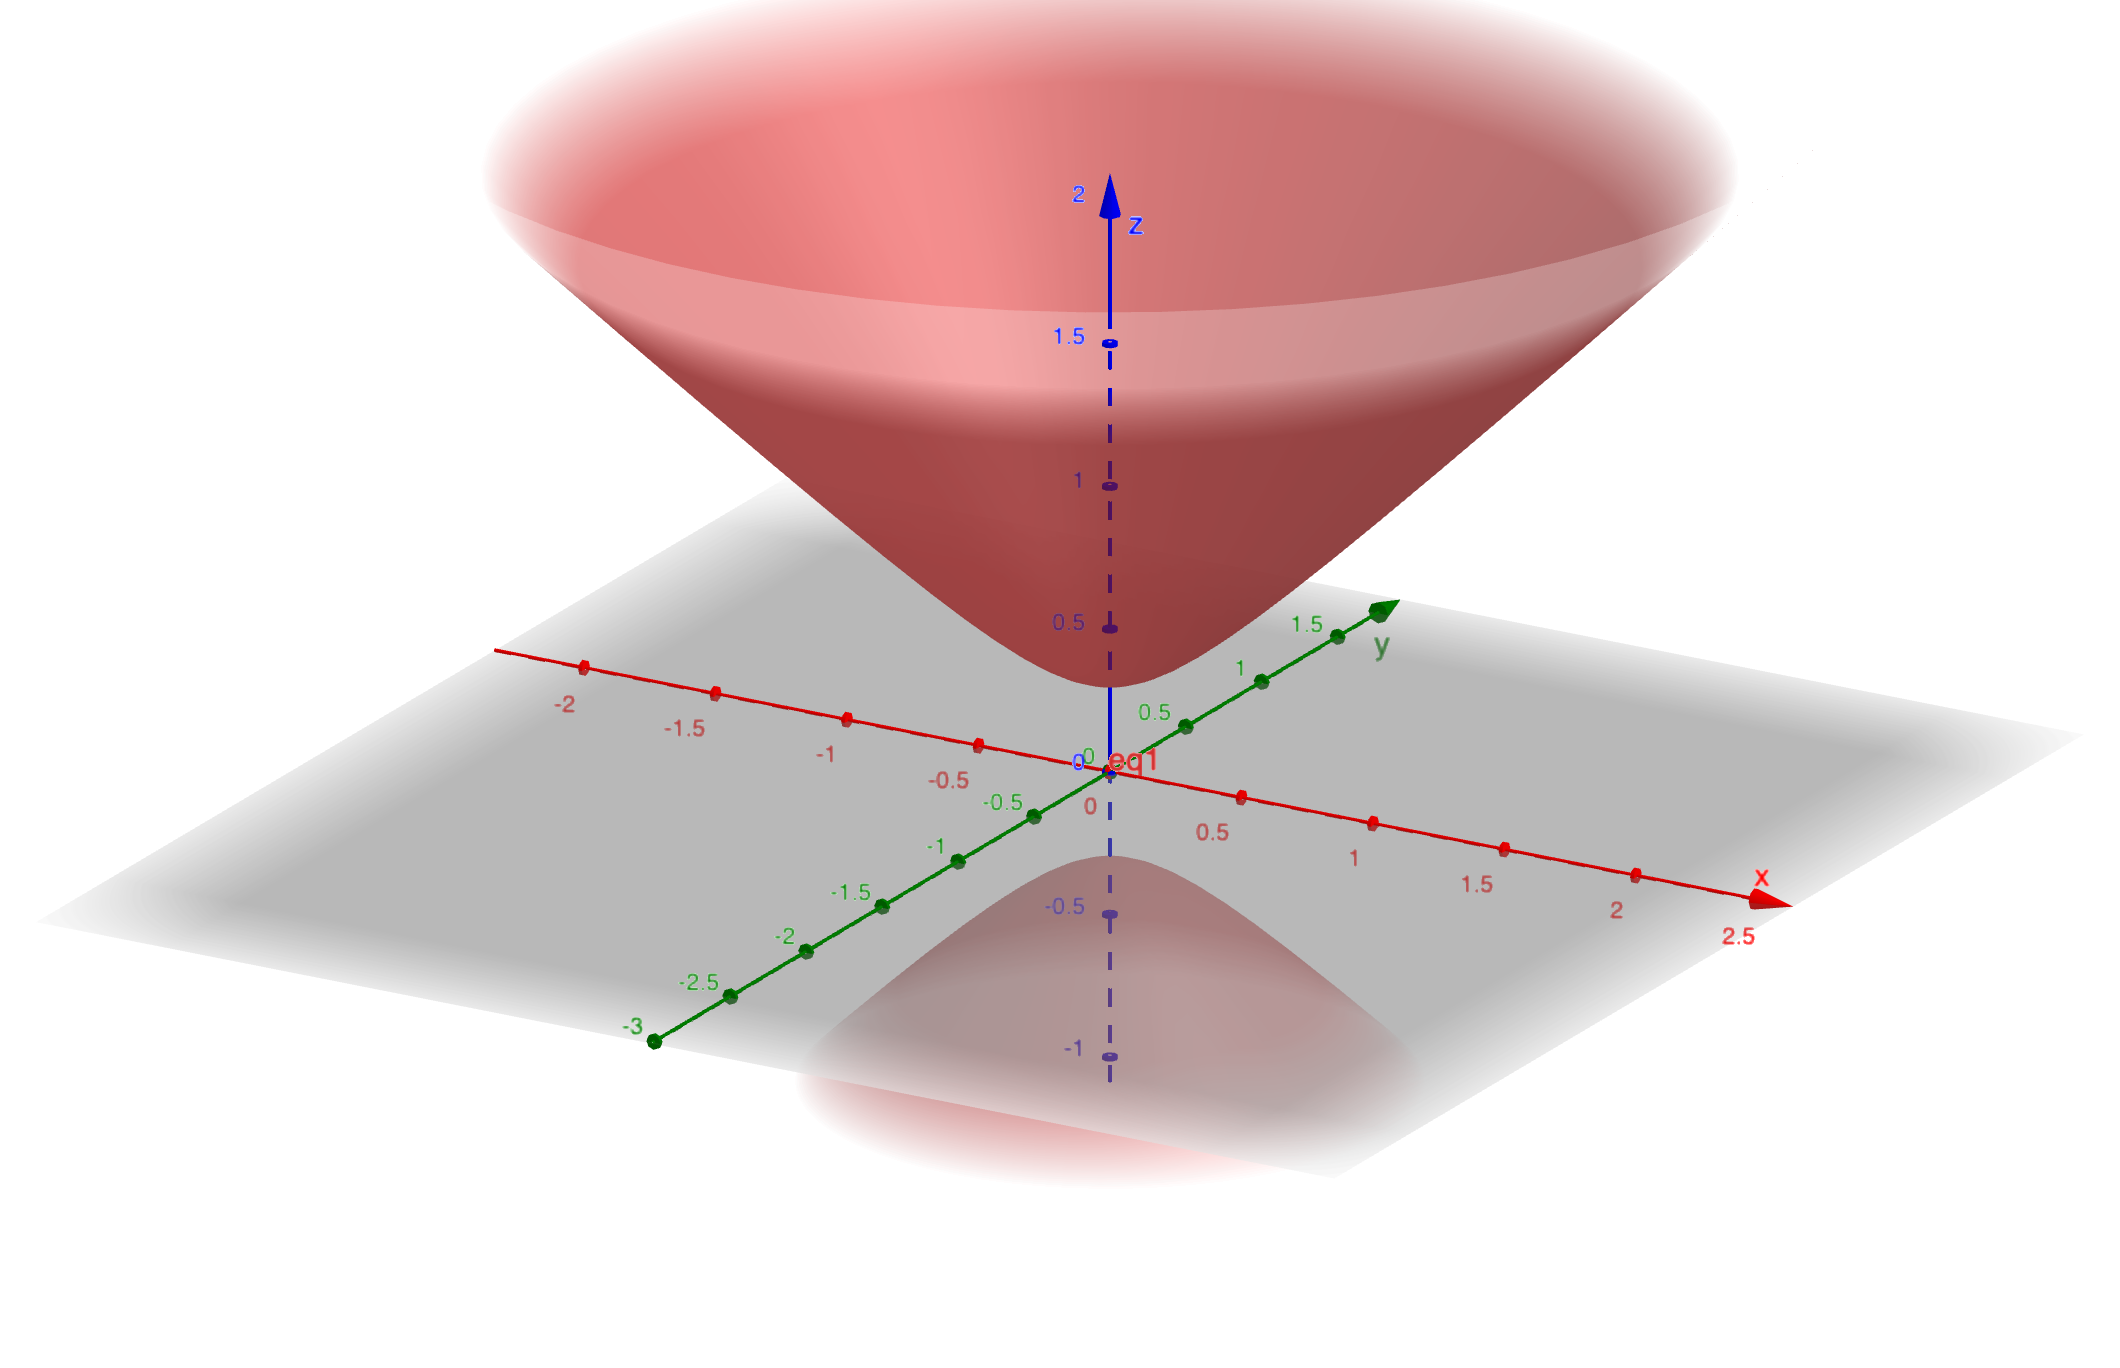
\includegraphics[width=.8\textwidth]{Figures_Part_6/hyperboloid_2_sheet.png}
                        \caption{Hyperboloid of 2-sheets defined by $c=-0.1$.}
                    \end{figure}
                \end{itemize}
                \end{ex}

                \begin{ex}{The Torus}{torus}
                For this example, I will choose specific nice numbers, but this is a yet another case of a level surface.  Take
                \[
                \left(3-\sqrt{x^2+y^2}\right)^2+z^2=\frac{3}{2}.
                \]
                This gives us the \emph{torus} with inner radius (the radius from the center of the donut hole to the center of the tube) $3=R$ and tube radius $\frac{3}{2}=r$. This looks like
                \begin{figure}[H]
                    \centering
                    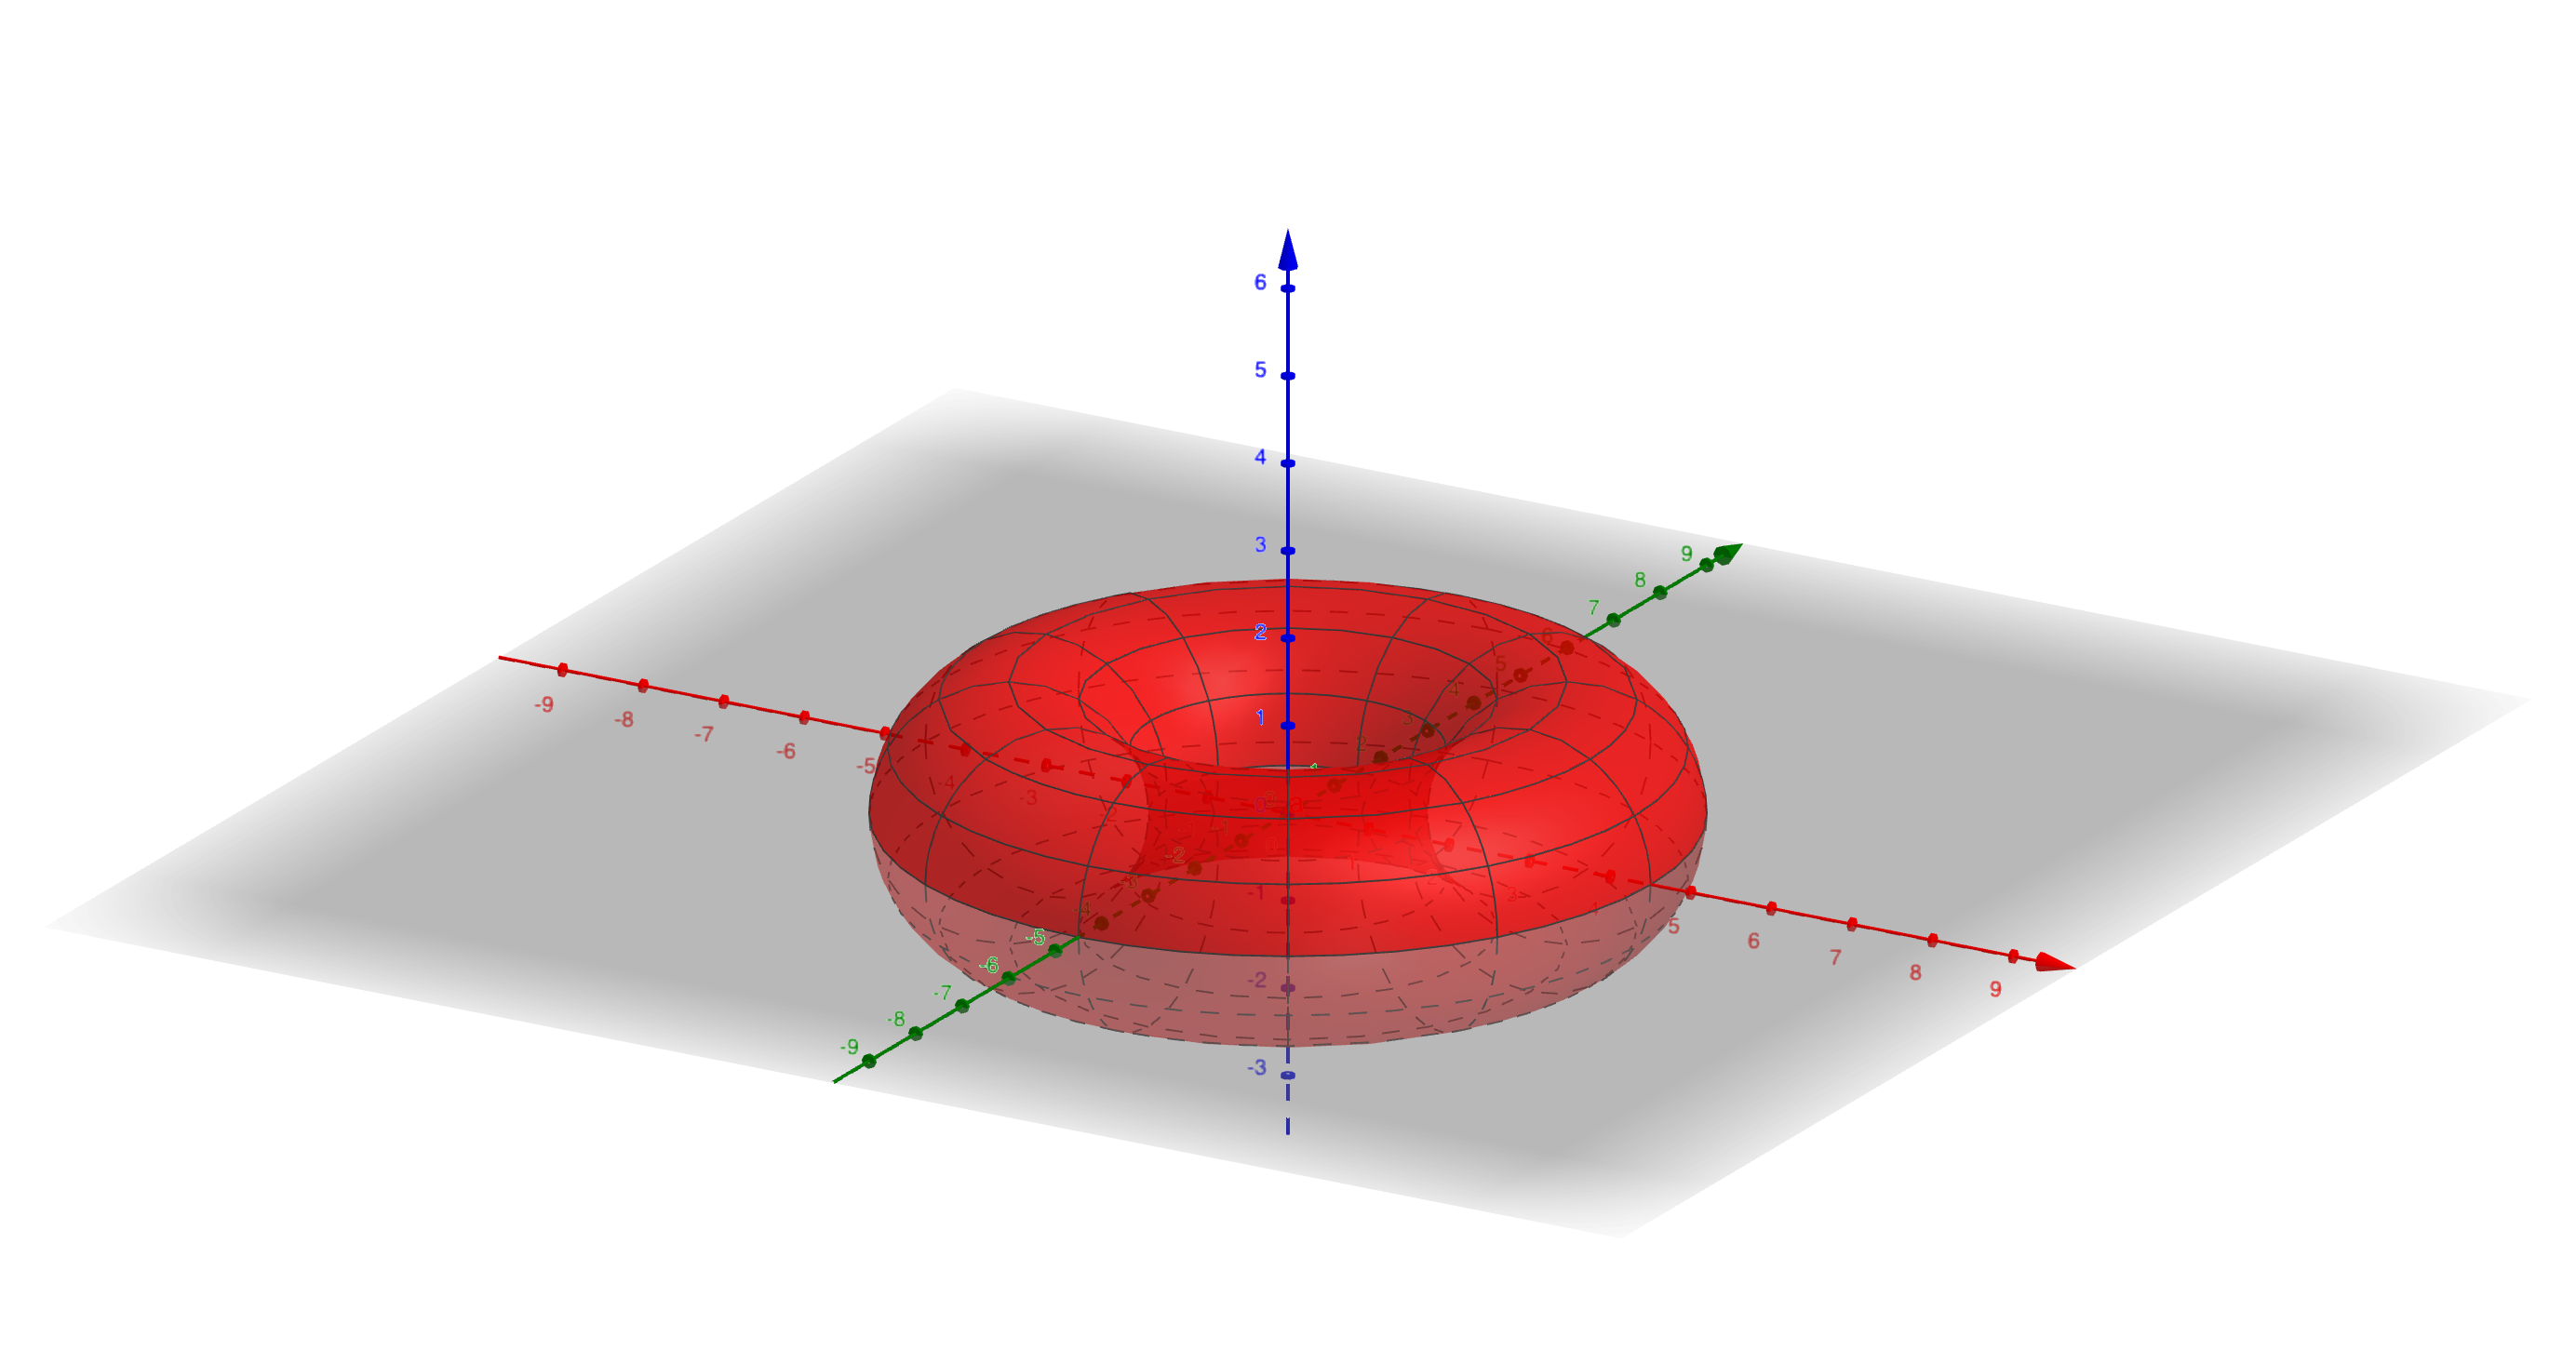
\includegraphics[width=.8\textwidth]{Figures_Part_6/torus.png}
                \end{figure}
                \end{ex}


                 \subsection{Normal Vectors to Implicit Surfaces}

                 Let $f(x,y,z)$ be a scalar field.  Then, recall that the gradient of this scalar function $\grad f$ points perpendicularly to the level sets of the scalar field.  Thus, if we have a level set of points for $f(x,y,z)=c$ and $\grad f \neq \zerovec$ at any of these points, then we have a means of describing the vector $\unitvec$ that is normal to the surface at each point.  Specifically, if the point $(x_0,y_0,z_0)$ are on the implicitly defined surface $f(x,y,z)=c$, then the normal vector at that point is given by
                 \[
                 \unitvec(x_0,y_0,z_0) = \frac{\grad f(x_0,y_0,z_0)}{|\grad f(x_0,y_0,z_0)|}.
                 \]

                 Previously, we wished to compute flux integrals of vector fields through surfaces.  But, we took the simplest cases of surfaces (specifically where the surfaces were flat and had a constant normal vector).  Now, we could conceivably compute flux integrals across implicitly defined surfaces!

                 One more step must be taken into account.  We must know how the the implicit function ``stretches" out our Cartesian coordinates.  Say, for example, we can solve for $z$ in our equation for the level surface $\Sigma$. That is, if we have $f(x,y,z)=c$, then we can solve for $z$ in terms of $x$ and $y$ to find $z=g(x,y)$.  Then, the area is stretched by a factor
                 \[
                 d\Sigma = \sqrt{ \left(\frac{\partial g}{\partial x}\right)^2 + \left(\frac{\partial g}{\partial y}\right)^2 +1 } dxdy.
                 \]
                 We will cover this in more depth later when we consider explicit surfaces.

                 \begin{ex}{Surface Normal to Unit Sphere}{surface_normal_to_sphere}
                 	Consider the unit sphere defined implicitly by the level set to
                 	\[
                 	f(x,y,z)=x^2+y^2+z^2 = 1.
                 	\]
                 	Then, we can compute the surface normal by taking
                 	\[
                 	\grad f = \begin{pmatrix} 2x \\ 2y \\ 2z \end{pmatrix}.
                 	\]
                 	Then, we also have that
                 	\[
                 	\left| \grad f \right| = \sqrt{4x^2+4y^2+4z^2} = 2 \sqrt{x^2+y^2+z^2}.
                 	\]
                 	Note that we are requiring that $x^2+y^2+z^1=1$ by definition, and thus
                 	\[
                 	\left| \grad f\right| = 2,
                 	\]
                 	along the unit sphere. Hence the surface normal to the unit sphere is given by
                 	\[
                 	\unitvec = \frac{\grad f}{\left| \grad f \right|} = \begin{pmatrix} x \\ y \\ z \end{pmatrix}.
                 	\]
                 	Thus, the surface normal to the sphere points in the same direction as the point on the sphere does!
                 \end{ex}

                 \begin{exercise}
                 	Plot the normal vectors to the unit sphere as well as the sphere.
                 \end{exercise}

                 \subsection{Implicit Function Theorem}

                 There is a great relationship between implicit surfaces and graphs of functions.  In general, graphs of functions are provide the nicest possible description of a surface.  Thus, one would appreciate the ability to be able to work with graphs while still defining a surface implicitly.

                 \begin{thm}{Implicit Function Theorem}
                 	Let $f(x,y,z)=c$ define an implicit surface.  Then where $\frac{\partial f}{\partial z}\neq 0$, we can describe the surface as the (possibly many) graph of functions $z=g(x,y)$. That is, the set of points $(x,y,g(x,y))$ describes a portion of the implicit surface.
                 \end{thm}

                 \begin{remark}
                 	There is in fact nothing special about the choice of graphing a function over the $xy$-plane.  One could instead have taken $\frac{\partial f}{\partial x} \neq 0$ and produced a graph $(g(y,z),y,z)$ instead! Given that, one could graph the surface over any plane in $\R^3$.
                 \end{remark}

                 This would not be a complete treatment if we did not provide an example for this.  So let us work through this description for the unit sphere.

                 \begin{ex}{The Sphere as Two Graphs}{sphere_graphs}
                 	Consider the unit sphere defined by
                 	\[
                 	f(x,y,z) = x^2+y^2+z^2 = 1.
                 	\]
                 	Then we have
                 	\[
                 	\frac{\partial f}{\partial z} = 2z,
                 	\]
                 	and hence as long as $z\neq 0$, we can build the unit sphere via graphs.  Specifically, we have
                 	\[
                 	z = \pm \sqrt{1-x^2-y^2}.
                 	\]
                 	Taking the graph $(x,y,\sqrt{1-x^2-y^2})$ yields the following.
                 	\begin{figure}[H]
                 		\centering
                 		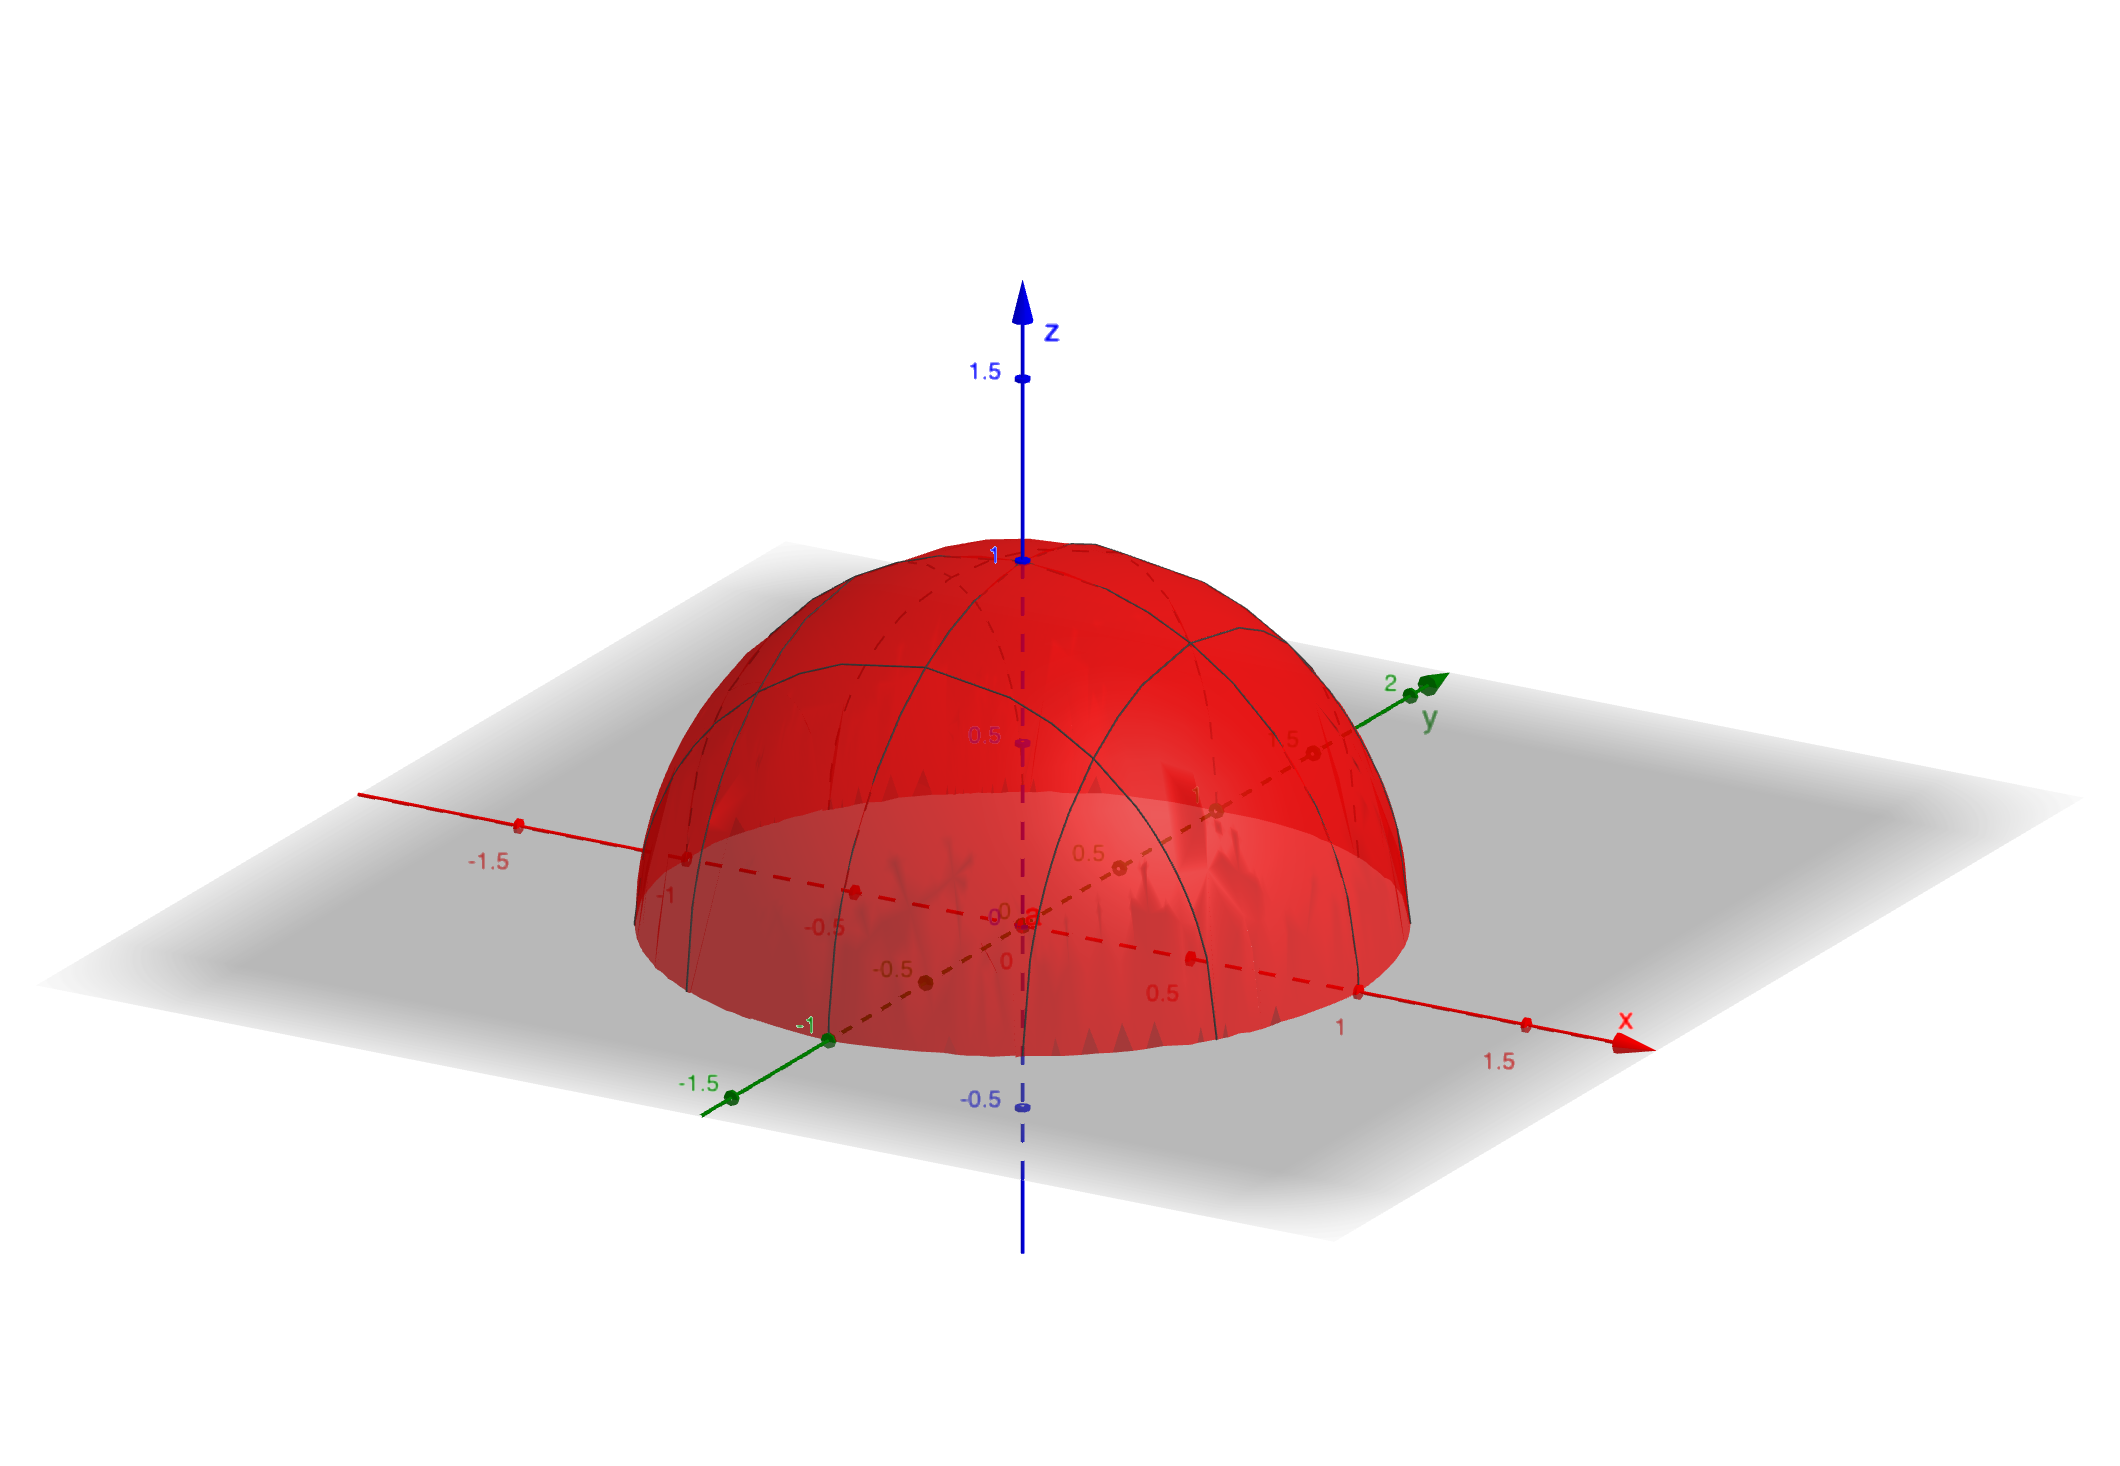
\includegraphics[width=.8\textwidth]{Figures_Part_6/hemisphere.png}
                 		\caption{The northern hemisphere given by the graph $(x,y,\sqrt{1-x^2-y^2})$.}
                 	\end{figure}
                 \end{ex}

                 \begin{exercise}
                 	Graph the other portion of the sphere by plotting $(x,y,-\sqrt{1-x^2-y^2})$ to see that the combination of these two graphs covers the whole sphere.
                 \end{exercise}

                 \section{Surfaces as Graphs}

                 Implicit surfaces provided a concise description for a surface as a level set of some scalar field.  One could then compute the surface normal.   However, to do further computations, it tends to be easiest to use an explicit description of a surface.  Luckily, the implicit function theorem provides us a means of construction a surface as a graph over the $xy$-plane (or really any other plane in $\R^3$).  So, it is worth continuing working with graphs of functions.

                 Suppose that we have a function $g(x,y)$ and we construct the surface $\Sigma$ given by the graph $(x,y,g(x,y))$.  One would like to construct the surface normal $\unitvec$ and compute the \boldgreen{area form} $d\Sigma$. Up until now, we have had no trouble defining $d\Sigma$ as our surfaces have been rather nice.

                 Our methodology for constructing these quantities will be to work very locally on a surface.  In other words, it is helpful to know what a surface looks like up very close.  In this case, the surface is best approximated by a plane.  This is analogous to how you can approximate functions of a single variable by a line.

                                        \begin{exercise}
                                        Compute the tangent line to $f(x)=2x^2+5$ at the point $x_0=3$.
                                        \end{exercise}

                                        \subsection{Equation for a Plane}

                                        We haven't worked much with planes in space yet, but we have seen surfaces.  In some sense, planes are the easiest surfaces.  They are, after all, linear objects.

                                        \begin{ex}{Plane and Normal}{plane_normal}
                                        The implicit equation for a plane is given by
                                        \[
                                        ax+by+cz+ d = 0.
                                        \]
                                        Notice that this is a linear equation.

                                        Then the surface normal to the plane is given by
                                        \[
                                        \unitvec = \frac{\grad f}{\left| \grad f\right|} = \frac{1}{\sqrt{a^2+b^2+c^2}}\begin{pmatrix} a \\ b \\ c\end{pmatrix}.
                                        \]
                                        We can see a diagram of this here.
                                        \begin{figure}[H]
                                            \centering
                                            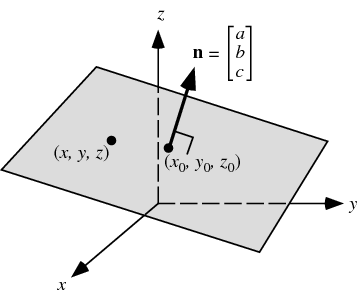
\includegraphics[width=.4\textwidth]{Figures_Part_6/plane_n.png}
                                        \end{figure}
                                        \end{ex}


                                        \subsection{Tangent Planes and Surface Normals}

                                        Now, if we are given a surface (defined as a level surface or as the graph of a function), we can compute an approximation at a point called the \boldgreen{tangent plane}. The means in which we compute this comes from computing the tangent vectors to curves along the surface.  If we have $\Sigma$ given by $(x,y,g(x,y))$, then we can create a curve along the surface aligned in the $x$-direction by letting $y$ be constant.  So, choose $y=k$ and we then have a curve given by the points
                                        \[
                                        \curvegamma_1(x) = \begin{pmatrix} x \\ k \\ g(x,k) \end{pmatrix}.
                                        \]
                                        Then, the tangent vector is given by
                                        \[
                                        \frac{d}{dx} \curvegamma_1(x) = \begin{pmatrix} 1 \\ 0 \\ \frac{\partial g}{\partial x} (x,k) \end{pmatrix} = \tangentgamma_1.
                                        \]
                                        In other words, we can simply compute a tangent vector in the $x$-direction on the graph by taking
                                        \[
                                        \frac{\partial}{\partial x} \begin{pmatrix} x \\ y \\ g(x,y) \end{pmatrix} = \begin{pmatrix} 1 \\ 0 \\ \frac{\partial g}{\partial x} \end{pmatrix}.
                                        \]
                                        Similarly, we can compute the tangent vector in the $y$-direction by
                                        \[
                                        \frac{\partial}{\partial y} \begin{pmatrix} x \\ y \\ g(x,y) \end{pmatrix} = \begin{pmatrix} 0 \\ 1 \\ \frac{\partial g}{\partial y} \end{pmatrix}.
                                        \]
                                        This gives us a means of computing the tangent plane in two ways. First, we have that the equation for the tangent plane to the graph of a function $g(x,y)$ at the point $(x_0,y_0,g(x_0,y_0))$ is given by
                                        \[
                                        z-g(x_0,y_0)=\frac{\partial g}{\partial x}(x_0,y_0)(x-x_0)+\frac{\partial g}{\partial y}(x_0,y_0)(y-y_0).
                                        \]
                                        Notice how this equation mimics the equation for a tangent line.  Similarly, we can compute the unit vector normal to the tangent plane by taking
                                        \[
                                        \unitvec = \frac{\tangentgamma_1 \times \tangentgamma_2}{\left| \tangentgamma_1 \times \tangentgamma_2\right|} = \frac{1}{\sqrt{1+\left(\frac{\partial g}{\partial x}\right)^2 + \left(\frac{\partial g}{\partial y}\right)^2}} \begin{pmatrix} -\frac{\partial g}{\partial x} \\ -\frac{\partial g}{\partial y} \\ 1 \end{pmatrix}.
                                        \]
                                     	It then follows that the vector normal to the tangent plane is indeed the surface normal at that point.  Thus, we have a nearly full description of the surface. Also, notice the denominator is very much related to the area form $d\Sigma$.  We'll work on computing this quantity next.

                                        \begin{ex}{Tangent Plane and Normal to a Paraboloid}
                                        Consider the function
                                        \[
                                        f(x,y)=-x^2-y^2.
                                        \]
                                        Then the graph of the function is given by plotting the points
                                        \[
                                        (x,y,f(x,y)).
                                        \]
                                        We compute the tangent plane by computing partial derivatives. We take
                                        \begin{align*}
                                        \frac{\partial f}{\partial x} &= -2x\\
                                        \frac{\partial f}{\partial y} &= -2y.
                                        \end{align*}
                                        Then the equation for a tangent plane at the point $(x_0,y_0,f(x_0,y_0))$ is given by
                                        \[
                                        z-f(x_0,y_0)=\partialx (x-x_0)+\partialy (y-y_0).
                                        \]
                                        So in our case, we have
                                        \[
                                        z-(-x_0^2-y_0^2)=-2x_0(x-x_0)-2y_0(y-y_0).
                                        \]
                                        Pictorially, it looks as follows (letting $p=(x_0,y_0,f(x_0,y_0))$):
                                        \begin{figure}[H]
                                            \centering
                                            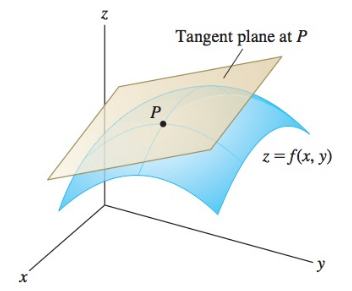
\includegraphics[width=.4\textwidth]{Figures_Part_6/tangent-planes-1.png}
                                        \end{figure}
                                        To compute the surface normal, we compute
                                        \[
                                        \tangentgamma_1 = \begin{pmatrix} 1 \\ 0 \\ -2x \end{pmatrix} \qquad \textrm{and} \qquad \tangentgamma_2 = \begin{pmatrix} 0 \\ 1 \\ -2y \end{pmatrix}.
                                        \]
                                        Computing the cross product yields,
                                        \[
                                        \begin{pmatrix} 2x \\ 2y \\ 1 \end{pmatrix},
                                        \]
                                        and we can normalize this vector by first computing
                                        \[
                                        \sqrt{1+(-2x)^2+(-2y)^2} = \sqrt{1-4x^2-4y^2}.
                                        \]
                                        Thus, our surface normal is given by
                                        \[
                                        \unitvec = \frac{1}{\sqrt{1-4x^2-4y^2}} \begin{pmatrix} 2x \\ 2y \\ 1 \end{pmatrix}.
                                        \]
                                        \end{ex}
   \section{Flux and Surface Integrals}

       	There was nothing too special about integrating over a curve, just as we saw with integration of scalar fields. In that case, we could integrate over any type of region that we would like.  Here, we can essentially do the same (one must be careful when the dimension not equal to three).  Fundamentally, what one would like to measure in the case of integration of a vector field $\vecfieldV$ over a surface $\Sigma$ is how much of the vector field passes through this surface.  If we have a surface $\Sigma$, then there is a unique (outward) normal vector to this surface denoted by $\unitvec$. That is, there is a unique vector that is perpendicular to the surface at that point. We can see this in the following figure.

       	\begin{figure}[H]
       		\centering
       		\def\svgwidth{0.75\columnwidth}
       		\input{Figures_Part_6/surface_normals.pdf_tex}
       	\end{figure}

       	 Keep in mind that the normal vector to a surface may change over time!  For example, the normal vector to a sphere will change, whereas the normal vector to a plane will not. This means that, in general, the normal vector is really a vector field $\unitvec(x,y,z)$. We will concentrate more on surfaces later, so for now we will take our surfaces to be planar.

       	The amount the vector field passes through the surface at the point $(x,y,z)$ is then given by the scalar quantity
       	\[
       	\vecfieldV(x,y,z) \cdot \unitvec(x,y,z).
       	\]
       	Then, if we integrate over the whole surface $\Sigma$ we have
       	\[
       	\iint_\Sigma  \vecfieldV \cdot \unitvec d\Sigma.
       	\]
        As we have seen, how we compute this will depend on the surface $\Sigma$. The picture for flux can be seen as follows.

               	\begin{figure}[H]
               		\centering
               		\def\svgwidth{0.75\columnwidth}
               		\input{Figures_Part_6/surface_flux.pdf_tex}
               	\end{figure}

         Above, the green arrows represent vectors coming from the vector field $\vecfieldV$ and the black arrows represent the surface normal $\unitvec$ at the corresponding point. By taking the dot product of the vector field with the unit vector at each point ($\vecfieldV(x,y,z)\cdot \unitvec(x,y,z)$) we compute the amount of the field flowing through that point.

        \begin{ex}{Total Flux Through a Plane}{flux_through_plane}
        	Consider the vector field $\vecfieldV(x,y,z) = \begin{pmatrix} x \\ y \\ z \end{pmatrix}$ and the planar surface $\Sigma$ given by $0\leq x \leq 1$, $2\leq y \leq 3$ and $z=5$.  Then, the normal to this surface is given by $\unitvec(x,y,z) = \begin{pmatrix} 0 \\ 0 \\ 1 \end{pmatrix} = \zhat.$ Note that we could have instead taken $-\unitvec$, but we chose the other orientation, and orientation is always a choice we can make.  Here, the normal vector does not change as we change our position in space.

        	We now wish to compute
        	\[
        	\iint_\Sigma \vecfieldV \cdot \unitvec d\Sigma.
        	\]
        	Now, given our surface defined above, we can put
        	\begin{align*}
        	\iint_\Sigma \vecfieldV \cdot \unitvec d\Sigma &= \int_2^3 \int_0^1 \vecfieldV(x,y,5) \cdot \zhat dxdy\\
        	&= \int_2^3 \int_0^1 5 dx dy\\
        	&= \int_2^3 5 dy\\
        	&= 5.
        	\end{align*}
        \end{ex}




                                      \section{Area Form and Integration}

                                      Let us begin this section by computing the area of the unit disk in the plane.  Specifically, this is the set of points inside the unit circle given by the equation $x^2+y^2\leq 1$.  How should we compute this area?

                                      \begin{ex}{Area of Unit Disk}{area_unit_disk}
                                      	Let the surface $\Sigma$ be the unit disk given by the set of points in the plane $x^2+y^2\leq 1$.  We know that the area should be $\pi$, and so if we integrate
                                      	\[
                                      	\iint_\Sigma d\Sigma,
                                      	\]
                                      	we should find this to be equal to the area of the unit disk.  In this case, since our surface is flat and in the $xy$-plane, we have that $d\Sigma = dxdy$, and so we just need to find our bounds of integration.  If we solve for $x$ in the given equation, we have
                                      	\[
                                      	\sqrt{x^2} \leq \sqrt{1-y^2},
                                      	\]
                                      	and note that $\sqrt{x^2}=|x|$ and thus this amounts to
                                      	\[
                                      	-\sqrt{1-y^2}\leq x \leq \sqrt{1-y^2}.
                                      	\]
                                      	\todo{insert figure}
                                      	So, as $y$ varies from $-1$ to $1$, this describes how $x$ should vary. So, we can write our integral as
                                      	\begin{align*}
                                      	\iint_\Sigma d\Sigma = \int_{-1}^1 \int_{-\sqrt{1-y^2}}^{\sqrt{1-y^2}} dxdy.
                                      	\end{align*}
                                      	We can compute this integral in the standard way
                                      	\begin{align*}
                                      	\int_{-1}^1 \int{-\sqrt{1-y^2}}^{\sqrt{1-y^2}} dxdy &= \int_{-1}^1 2\sqrt{1-y^2}dy\\
                                      	&= \pi.
                                      	\end{align*}
                                      	This is the correct area of the unit disk.
                                      \end{ex}

                                      \begin{exercise}
                                      Fill in the gaps in the integral for the previous example.
                                      \end{exercise}

                                      Lastly, we need to describe the area form $d\Sigma$.  The idea of $d\Sigma$ is to capture the ``stretching" that occurs when we graph a function.  Geometrically, what we are doing when we take the graph of a function is we are taking a region in the plane, and applying a function to this region that lifts the area up and stretches it into the desired surface.  For example, if we take the unit disk in the plane given by the set of points $(x,y)$ satisfying $x^2+y^2\leq 1$.  Then, we can create the northern hemisphere surface by taking the graph $(x,y,\sqrt{1-x^2-y^2})$.  Through this process, the unit disk is transformed into the northern hemisphere.  One can note that the area of the unit disk is $\pi$ and the area of the northern hemisphere of the unit sphere is $2\pi$.  So, it must be that this act of graphing deforms area!

                                      We want to know how the area is deformed at every single point on our surface, and so we need a way to compute this.  Recall that the cross product of two vectors in $\R^3$ gives us the area of the parallelogram defined by the two vectors.  Specifically, if we have $\vecu,\vecv \in \R^3$, then the area of the parallelogram is given by $A=|\vecu\times \vecv|$.  Thinking along these lines, if we can compute an infinitesimal parallelogram on our surface, we can compute what the area is.  Specifically, what we will do is take an infinitesimal movement along our surface $x$-direction and $y$-direction, and see what the area given by these infinitesimal vectors will be.  In other words, we want to compute an infinitesimal version of
                                      \[
                                      |\tangentgamma_1 \times \tangentgamma_2|,
                                      \]
                                      where $\tangentgamma_1$ and $\tangentgamma_2$ are tangent vectors at the point of interest.  Recall that
                                      \[
                                      \tangentgamma_1 = \begin{pmatrix} 1 \\ 0 \\ \frac{\partial g}{\partial x} \end{pmatrix}  \qquad \textrm{and} \qquad  \tangentgamma_2 = \begin{pmatrix} 0 \\ 1 \\ \frac{\partial g}{\partial y} \end{pmatrix}.
                                      \]
                                      We can make these of infinitesimal lengths by taking the $x$-coordinate to be the infinitesimal $dx$, the $y$-coordinate to $dy$, and the $z$-coordinate to be $dz$.  Hence, we want to compute
                                      \[
                                      \left| \begin{pmatrix} dx \\ 0 \\ dz \end{pmatrix} \times \begin{pmatrix} 0 \\ dy \\ dz \end{pmatrix} \right|.
                                      \]
                                      However, we can note that $z=g(x,y)$ is a function. Thus, we can write $dz$ in terms of $dx$ and $dy$.  Specifically, we can compute the \boldgreen{differential}
                                      \[
                                      dz = \frac{\partial g}{\partial x}dx + \frac{\partial g}{\partial y}dy.
                                      \]
                                      Let us pause briefly to define this.

                                      \begin{df}{Differential of a Scalar Field}{differential}
                                      	Given a scalar field $f(x,y,z)$, the \emph{differential} $df$ is given by
                                      	\[
                                      	df = \frac{\partial f}{\partial x}dx + \partialy dy + \partialz dz.
                                      	\]
                                      \end{df}

                                     Returning to our work before, we were wishing to compute
                                     \[
                                     \left| \begin{pmatrix} dx \\ 0 \\  \frac{\partial g}{\partial x}dx + \frac{\partial g}{\partial y}dy \end{pmatrix} \times \begin{pmatrix} 0 \\ dy \\  \frac{\partial g}{\partial x}dx + \frac{\partial g}{\partial y}dy \end{pmatrix}\right|.
                                     \]
                                     Computing this cross product yields
                                     \[
                                     \left| \begin{pmatrix} -\frac{\partial g}{\partial x} dydz \\ \frac{\partial g}{\partial y}dxdz \\ dxdy \end{pmatrix} \right|.
                                     \]
                                     Let us compute further,
                                    \begin{align*}
                                     \begin{pmatrix} -\frac{\partial g}{\partial x} dydz \\ \frac{\partial g}{\partial y}dxdz \\ dxdy \end{pmatrix} &= \begin{pmatrix} -\frac{\partial g}{\partial x}dxdy - \frac{\partial g}{\partial y} dy^2 \\ \frac{\partial g}{\partial x}dx^2+\frac{\partial g}{\partial y} dxdy \\ dxdy \end{pmatrix}.
                                    \end{align*}
                                    Now, if we are trying to compute area, then the area generated by $dx^2$ is 0 since no area is contained in this infinitesimal parallelogram. Likewise $dy^2=0$ as well. Hence, our result is
                                    \[
                                    \begin{pmatrix} -\frac{\partial g}{\partial x} dxdy \\ \frac{\partial g}{\partial y} dxdy \\ dxdy \end{pmatrix}.
                                    \]
                                    Then, computing the length of this vector yields
                                     \begin{align*}
                                     \left| \begin{pmatrix} -\frac{\partial g}{\partial x} dxdy \\ \frac{\partial g}{\partial y} dxdy \\ dxdy \end{pmatrix}\right| &= \sqrt{ \left( \frac{\partial g}{\partial x}  \right)^2 (dxdy)^2 + \left( \frac{\partial g}{\partial y} \right) (dxdy)^2 + (dxdy)^2}\\
                                     &= \sqrt{\left(\frac{\partial g}{\partial x} \right)^2 + \left( \frac{\partial g}{\partial y}  \right)^2 +1 } dxdy.
                					\end{align*}
                					Thus, after this tedious computation, we have that for a surface defined by a graph
                					\[
                					d\Sigma = \sqrt{\left(\frac{\partial g}{\partial x} \right)^2 + \left( \frac{\partial g}{\partial y}  \right)^2 +1 } dxdy.
                					\]

                                     \begin{ex}{Area form on the Northern Hemisphere}{area_form_hemisphere}
                                     	Consider the graph of the northern hemisphere given by
                                     	\[
                                     	(x,y,\sqrt{1-x^2-y^2}),
                                     	\]
                                     	for $x$ and $y$ values satisfying $x^2+y^2\leq 1$.  Letting $g(x,y)=\sqrt{1-x^2-y^2}$, we have that
                                     	\[
                                     	\frac{\partial g}{\partial x} = -\frac{x}{\sqrt{1-x^2-y^2}} \qquad \textrm{and} \qquad \frac{\partial g}{\partial y} = -\frac{y}{\sqrt{1-x^2-y^2}}.
                                     	\]
                                     	Then we have
                                     	\begin{align*}
	                                     	d\Sigma = \sqrt{\left(\frac{\partial g}{\partial x}\right)^2 + \left(\frac{\partial g}{\partial y}\right)^2 + 1 }dxdy\\
	                                     	&=\sqrt{\frac{1}{1-x^2-y^2}}dxdy.
                                     	\end{align*}
                                     	If we have computed this correctly, then we should have that the surface area of the northern hemisphere is given by
                                     	\[
                                     	\iint_\Sigma d\Sigma.
                                     	\]
                                     	Now, we require that $x^2+y^2\leq 1$, and we can find
                                     	\[
                                     	\sqrt{x^2}\leq \sqrt{1-y^2},
                                     	\]
                                     	which means that
                                     	\[
                                     	-\sqrt{1-y^2}\leq x \leq \sqrt{1-y^2},
                                     	\]
                                     	as $y$ ranges from $-1$ to $1$.  Hence, we have that
                                     	\[
                                     	\iint_\Sigma d\Sigma = \int_{-1}^1 \int_{-\sqrt{1-y^2}}^{\sqrt{1-y^2}} \sqrt{\frac{1}{1-x^2-y^2}}dxdy = 2\pi,
                                     	\]
                                     	which is indeed the area of the northern hemisphere.
                                     \end{ex}

                                     \begin{remark}
                                     	The above integral is rather hard to compute in Cartesian coordinates.  Thus, we will be motivated to choose a different way of computing that integral to simplify this problem.
                                     \end{remark}

                                     Now, if we are solely integrating along a surface defined by a graph, then notice that we have the following nice relationship.  We have that
                                     \begin{align*}
                                     \unitvec d\Sigma &= \frac{\tangentgamma_1\times \tangentgamma_2}{\left|\tangentgamma_1 \times \tangentgamma_2\right|} \left|\tangentgamma_1 \times \tangentgamma_2 \right| dxdy\\
                                     &= \left(\tangentgamma_1 \times \tangentgamma_2\right)dxdy\\
                                     &= \begin{pmatrix} -\frac{\partial g}{\partial x} \\ -\frac{\partial g}{\partial y} \\ 1 \end{pmatrix} dx dy.
                                     \end{align*}
                                      Putting this together with the previous section, we can compute a nice example.

                                   	\begin{ex}{Flux Through Northern Hemisphere}{flux_through_northern_hemisphere}
                                   		Consider the vector field
                                   		\[
                                   		\vecfieldV(x,y,z) = \begin{pmatrix}  x\\ y \\ z \end{pmatrix},
                                   		\]
                                   		and the graph of the northern hemisphere surface $\Sigma$ given by $(x,y,g(x,y))$ where
                                   		\[
                                   		g(x,y) = \sqrt{1-x^2-y^2}.
                                   		\]
                                   		We want to integrate
                                   		\[
                                   		\iint_\Sigma \vecfieldV \cdot \unitvec d\Sigma.
                                   		\]
                                   		Then, we have computed the normal vector to the whole unit sphere to be
                                   		\[
                                   		\unitvec = \begin{pmatrix} x \\ y \\ z \end{pmatrix}
                                   		\]
                                   		as well as the area form
                                   		\[
                                   		d\Sigma = \sqrt{\frac{1}{1-x^2-y^2}}dxdy.
                                   		\]
                                   		Along this surface.  Thus, we have
                                   		\begin{align*}
                                   			\iint_\Sigma \vecfieldV \cdot \unitvec d\Sigma &= \int_{-1}^1 \int_{-\sqrt{1-y^2}}^{\sqrt{1-y^2}} \begin{pmatrix} x \\ y \\ z \end{pmatrix} \cdot \begin{pmatrix} x \\ y \\ z \end{pmatrix} \sqrt{\frac{1}{1-x^2-y^2}}dxdy\\
                                   			&= \int_{-\sqrt{1-y^2}}^{\sqrt{1-y^2}} (x^2+y^2+z^2) \sqrt{\frac{1}{1-x^2-y^2}}dxdy.
                                   		\end{align*}
                                   		Note that along the unit sphere we have that $x^2+y^2+z^2=1$, and thus our integral reduces to
                                   		\[
                                   		\iint_\Sigma \vecfieldV \cdot \unitvec d\Sigma =  \int_{-\sqrt{1-y^2}}^{\sqrt{1-y^2}} \sqrt{\frac{1}{1-x^2-y^2}}dxdy.
                                   		\]
                                   		To evaluate this integral, we will learn to use different coordinates!
                                   	\end{ex}

                                   	In summary, if a surface is given as a graph, we have all the tools to integrate.  One should then revisit the idea of integrating over a implicit surface. Notice in that case, we can define the surface using multiple graphs, and so this reduces to integrating along each necessary graph.

%                                        \begin{ex}{Flux Through Sphere}{flux_through_sphere}
%                                                         Consider the vector field
%                                                         \[
%                                                         \vecfieldV(x,y,z) = \begin{pmatrix} x \\ y \\ z \end{pmatrix}
%                                                         \]
%                                                          and the unit sphere surface $\Sigma$ given by
%                                                          \[
%                                                          f(x,y,z)=x^2+y^2+z^2=1.
%                                                          \]
%                                                          Then, we wish to compute the following integral
%                                                          \[
%                                                          \iint_\Sigma \vecfieldV \cdot \unitvec d\Sigma.
%                                                          \]
%                                                          First, note that we have that
%                                                          \[
%                                                          \unitvec = \frac{\grad f}{|\grad f|} = \frac{1}{\sqrt{4x^2+4y^2+4z^2}} \begin{pmatrix} 2x \\ 2y \\ 2z \end{pmatrix}.
%                                                          \]
%                                                          Then, since we are on the unit sphere we have $x^2+y^2+z^2=1$, and thus
%                                                          \[
%                                                          \unitvec = \begin{pmatrix} x \\ y \\ z \end{pmatrix},
%                                                          \]
%                                                          for any point on the unit sphere.  Now, we can solve for $z$ in the above equation to find
%                                                          \[
%                                                          z = \pm \sqrt{1-x^2-y^2} = g(x,y),
%                                                          \]
%                                                          and so our integral will split up into the integral over two graphs of functions (which we know how to do).  Then, we have that
%                                                          \begin{align*}
%                                                          d\Sigma &= \sqrt{ \left(\frac{\partial g}{\partial x}\right)^2 + \left(\frac{\partial g}{\partial y}\right)^2 +1 } dxdy\\
%                                                          &= \sqrt{\frac{x^2}{1-x^2-y^2}+\frac{y^2}{1-x^2-y^2}+1}dxdy\\
%                                                          &= \sqrt{\frac{1}{1-x^2-y^2}}dxdy
%                                                          \end{align*}
%
%                                                          That is, we have the integral over the northern hemisphere
%                                                          \begin{align*}
%                                                          \int_{-1}^1 \int_{-1}^1 \begin{pmatrix} x \\ y \\ z \end{pmatrix} \cdot \begin{pmatrix} x \\ y \\ z \end{pmatrix} \left(1-x^2-y^2\right)dxdy &= \int_{-1}^1 \int_{-1}^1 \left( x^2 + y^2 +z^2\right) \left(1-x^2-y^2\right)dxdy\\
%                                                          &= \int_{-1}^1 \int_{-1}^1 \frac{1}{\sqrt{1-x^2-y^2}}dxdy.
%                                                          \end{align*}
%                                                          Simimlarly, the southern hemisphere has the same value, and thus we have
%                                                          \[
%                                                          \iint_{\Sigma} \vecfieldV \cdot \unitvec d\Sigma = 2 \int_{-1}^1 \int_{-1}^1 \frac{1}{\sqrt{1-x^2-y^2}}dxdy.
%                                                          \]
%                                                          One could then evaluate this integral using a change of variables and trigonometric integration.
%                                                         \end{ex}
%


